%% Copyright 1998 Pepe Kubon
%%
%% `one.tex' --- 1st chapter for thes-full.tex, thes-short-tex from
%%                the `csthesis' bundle
%%
%% You are allowed to distribute this file together with all files
%% mentioned in READ.ME.
%%
%% You are not allowed to modify its contents.
%%

%%%%%%%%%%%%%%%%%%%%%%%%%%%%%%%%%%%%%%%%%%%%%%%%%
%
%       Chapter 1 
%
%%%%%%%%%%%%%%%%%%%%%%%%%%%%%%%%%%%%%%%%%%%%%%%%

\chapter{Introduction}\label{chap:one}
Detection of outliers is an essential part of knowledge discovery in databases (KDD) and has been used to identify  anomalous entities from data for decades. System faults or changes, human or mechanical error, or any sort of deviations in population caused by unknown reasons, may result in outliers in the data \cite{Hodge2004}.\\
Many techniques have been employed in Data Mining, Machine Learning, and Statistics to find outliers in different domains such as Network Performance, Motion Segmentation, Medical Condition Monitoring and Pharmaceutical Research. Demand for efficient analysis methods to detect outliers has been increased due to the large amount of data collected in databases. In this dissertation, we developed two generative model-based methods for the case of object-relational data. 

\section{Outlier Definition}\label{sec:outdefinition}

Many definitions have been proposed for an outlier and there is no generally accepted definition. Grubbs {\em et al.} define an outlier as an observation that appears to deviate considerably from other members of the sample in which it occurs~\cite{grubbs1969}. Hawkings {\em et al.} describe an outlier as an observation which deviates so much from the other observations as to arouse suspicions that it was generated by a different mechanism~\cite{Hawkins1980}. These are only a few examples of definitions proposed in the previous outlier detection work. Essentially, the outlier definition is context-related and depends on the type of the application that employs the outlier detection.  For example, Akoglu {\em et. al} define outliers in graphs as rare graph objects that differ significantly from the majority of the reference objects in the graph~\cite{Akoglu2010}. This definition is the basis of our proposed outlier detection methods.  

%\subsection{Types of Outlier}
%Outliers have been categorized into three classes: global outliers, contextual (or conditional) outliers and collective outliers~\cite{Han2011}. 
%\paragraph{ Global Outlier}
%Whenever a data point notably deviates from the rest of population, it is categorized as {\em global outlier} (Figure~\ref{fig:Outlier-Type}a). This type of outliers are the simplest and finding them is the target of most of outlier detection methods. The main challenge of this type of outlier is that sometimes it is hard to find an appropriate measurement of deviation.
%
%\begin{figure*}%[!htbp]
%	\centering
%	\resizebox{0.8\textwidth}{!}{
%		\includegraphics%[width=0.3\textwidth] 
%		{figures/outlierType-c.pdf}
%	}
%	\caption{Global outlier vs. Collective outlier
%		\label{fig:Outlier-Type}}
%\end{figure*}
%
%\paragraph{ Contextual Outlier}
%
%An object is an outlier if it deviates notably based on selected context. For example if the question is whether temperature $20\,^{\circ}{\rm C}$ is abnormal for Toronto depends on whether it is summer or winter. Attributes of data points are divided into two groups: {\em contextual attributes}: defines the context e.g., time and location. {\em Behavioral attributes} e.g.\ temperature are characteristics of the object, used in outlier evaluation. When we don't have any contextual attributes in our datasets, global outliers can be viewed as a special case of contextual outliers. The challenge of this type of outlier is to define and formulate context and requires great knowledge of domain~\cite{aggarwal2013}.
%\paragraph{ Collective Outlier}
%In this type of outlier, a subset of data points collectively deviates from the population. None of the individual data points may be outliers. Such collective anomalies typically represent unusual events, which need to be discovered from the data. For example, when number of computers start sending denial-of-service packages to each other, it can be result of an intrusion. 
%In  this type of outliers, focus is not only on behavior of individual data points, but also on group of the objects (see ~Figure \ref{fig:Outlier-Type}b).\\
The output of an outlier detection algorithm can be one of these two types~\cite{aggarwal2013}: 
\begin{enumerate}
	\item Outlier score assigned to each individual that shows the degree of ``outlierness" of each data point.
	\item A binary label indicating whether a data point is an outlier or not. By imposing thresholds on outlier scores, based on their statistical distribution, the outlier scores can be converted into binary labels.
\end{enumerate}
\subsection{Outlier Detection Challenges}
Outlier Detection applications must overcome many challenges. For example: 
\begin{itemize}
	\item Modeling normality is hard:
	there is not often a clear line separating data normality and abnormality since it is hard to define all possible normal behaviours. Therefore, many outlier techniques measure the degree of outlier-ness of each data point instead of firmly labelling it as either outlier or normal.
	\item Designing an outlier detection method depends on the type of application: one of the earliest steps in designing a model to identify outliers is choosing similarity or distance measure. However, different applications require different sensibility in terms of similarity or difference. For example, in medical data analysis, a tiny deviation may be a sign of an outlier; while marketing analysis, for example, allows larger fluctuations between its normal data points.
	\item Separating noise and error from the outliers: outliers and noise are different, however, they are similar in the sense that they both deviate from the normal behaviour. This similarity can make the distinction between normal and outlier and noise objects even harder.
	\item Understandability and interpretability: in some applications, detected outliers should be justified and the features that moved the data points from normal to outlier should be identified. In this case, outlier detection methods must provide some explanations. 
	\item Class imbalance: the imbalanced nature of outlier detection makes accurate detection hard to achieve.

\end{itemize}


%\paragraph{Bayesian Network}
%A class-model Bayes net (BN) structure is learned with data for the entire population. The nodes in the BN represent attributes for links, of multiple types, and attributes of entities, also of multiple types.
%A {\bf Bayesian Network (BN)} is a directed acyclic graph (DAG) whose nodes comprise a set of random variables \cite{Pearl1988}. Depending on context, we interchangeably refer to the nodes  and variables of a BN. Fix a set of variables $\Features = \{\feature_{1},\ldots,\feature_{n}\}$. 
%%These are attributes of objects, which can and typically do belong to different classes. In statistical terms, each attribute defines a random variable. 
%The possible values of $\feature_{i}$ are enumerated as $\{\nodevalue_{i1},\ldots,\nodevalue_{i\states_{i}}\}$. The notation $P(\feature_{i} = \nodevalue)\equiv P(\nodevalue)$ denotes the probability of variable $\feature_{i}$ taking on value $\nodevalue$. We also use the vector notation $P(\Features = \set{\nodevalue}) \equiv P(\set{\nodevalue})$ to denote the joint probability that each variable $\feature_{i}$ takes on value $\set{\nodevalue}_{i}$. 
%The conditional probability parameters of a Bayesian network specify the distribution of a child node given an assignment of values to its parent node. For an assignment of values to its nodes, a BN defines the joint probability as the product of the conditional probability of the child given its parent values, for each child node in the network. This means that the log-joint probability can be {\em decomposed} as the node-wise sum
%
%\begin{equation} \label{eq:bn}
%\ln P(\Features = \set{\nodevalue};\model,\parameters) = \sum_{i=1}^{n} \ln \parameter(\set{\nodevalue}_{i}|\set{\nodevalue}_{\parents_{i}})
%\end{equation}
%where $\set{\nodevalue}_{i}$ resp. $\set{\nodevalue}_{\parents_{i}}$ is the assignment of values to node $i$ resp. the parents of $i$ determined by the assignment $\set{\nodevalue}$. 
%%The function $\ln$ is the binary logarithm base 2. 
%To avoid difficulties with $\ln(0)$, here and below we assume that joint distributions are positive everywhere. Since the parameter values for a Bayes net define a joint distribution over its nodes, they therefore entail a marginal, or unconditional, probability for a single node. We denote the \textbf{marginal probability} that node $\feature$ has value $\nodevalue$ as $P(\feature = \nodevalue;\model,\parameters) \equiv \parameter(\nodevalue)$.

%\paragraph{Example.} Figure~\ref{fig:propositionalize} shows an example of a Bayesian network and associated joint and marginal probabilities.
%\begin{figure*}[htbp]
%	\centering
%	\includegraphics[width=0.5\textwidth]{figures/bn.pdf}
%	\caption{Example of joint and marginal probabilities computed from a toy Bayesian Network structure
%		\label{fig:propositionalize}}
%\end{figure*}
%\begin{figure}[!htbp]
	
%	\begin{minipage}{.5\linewidth}
%		\centering
%		\subfloat[A tree structure for related work on outlier detection for structured data. A path specifies an outlier detection problem, the leaves list major approaches to the problem. Stars show the proposed approaches in this thesis proposal ]{\label{main:a}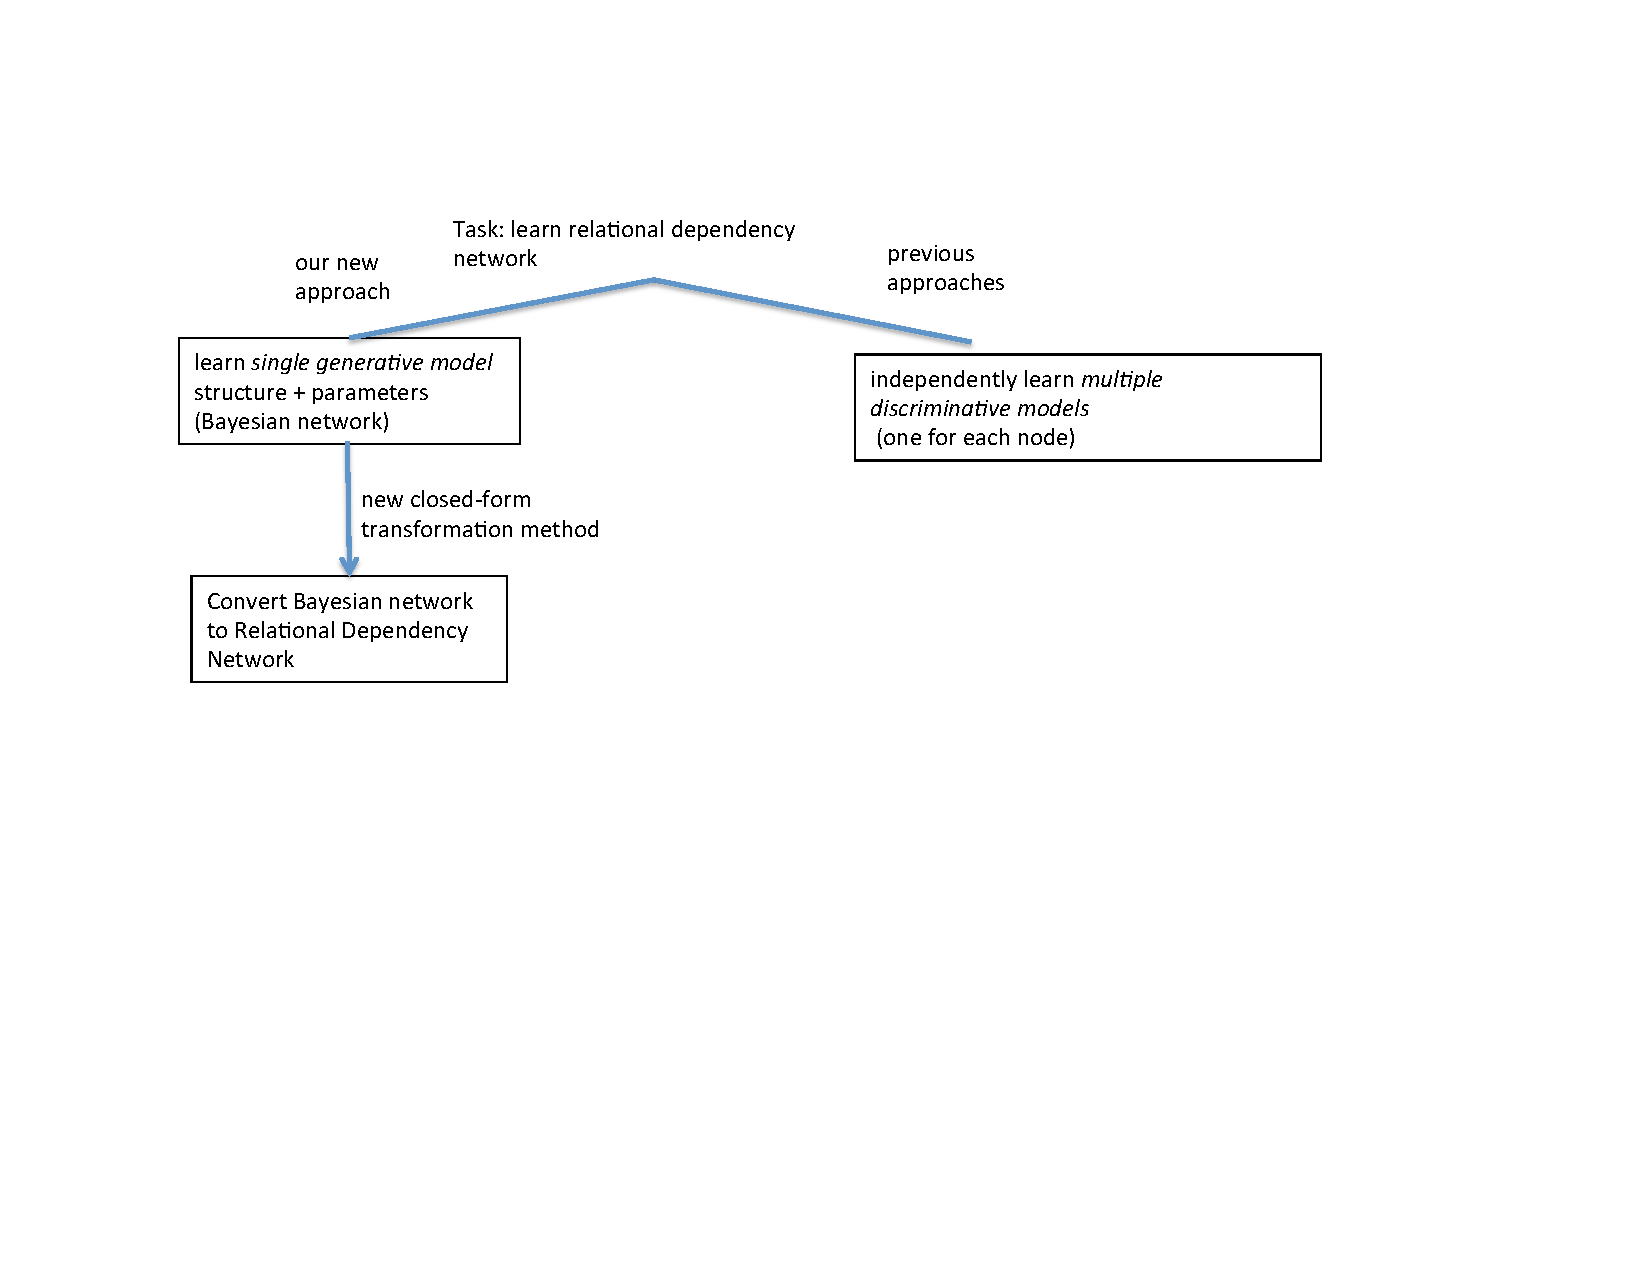
\includegraphics[scale=.45]{novelty.pdf}}
%	\end{minipage}%
%	\begin{minipage}{.75\linewidth}
%		\centering
%		\subfloat[Example of joint and marginal probabilities computed from a toy Bayesian Network structure]{\label{main:b}\includegraphics[scale=.40]{bn.pdf}}
%	\end{minipage}\par\medskip
%	\caption{}
%	\label{fig:propositionalize}
%\end{figure}
%\begin{figure}[!htbp]
%	
%	\begin{minipage}{.5\linewidth}
%		\centering
%		\subfloat[An example database]{\label{main:a}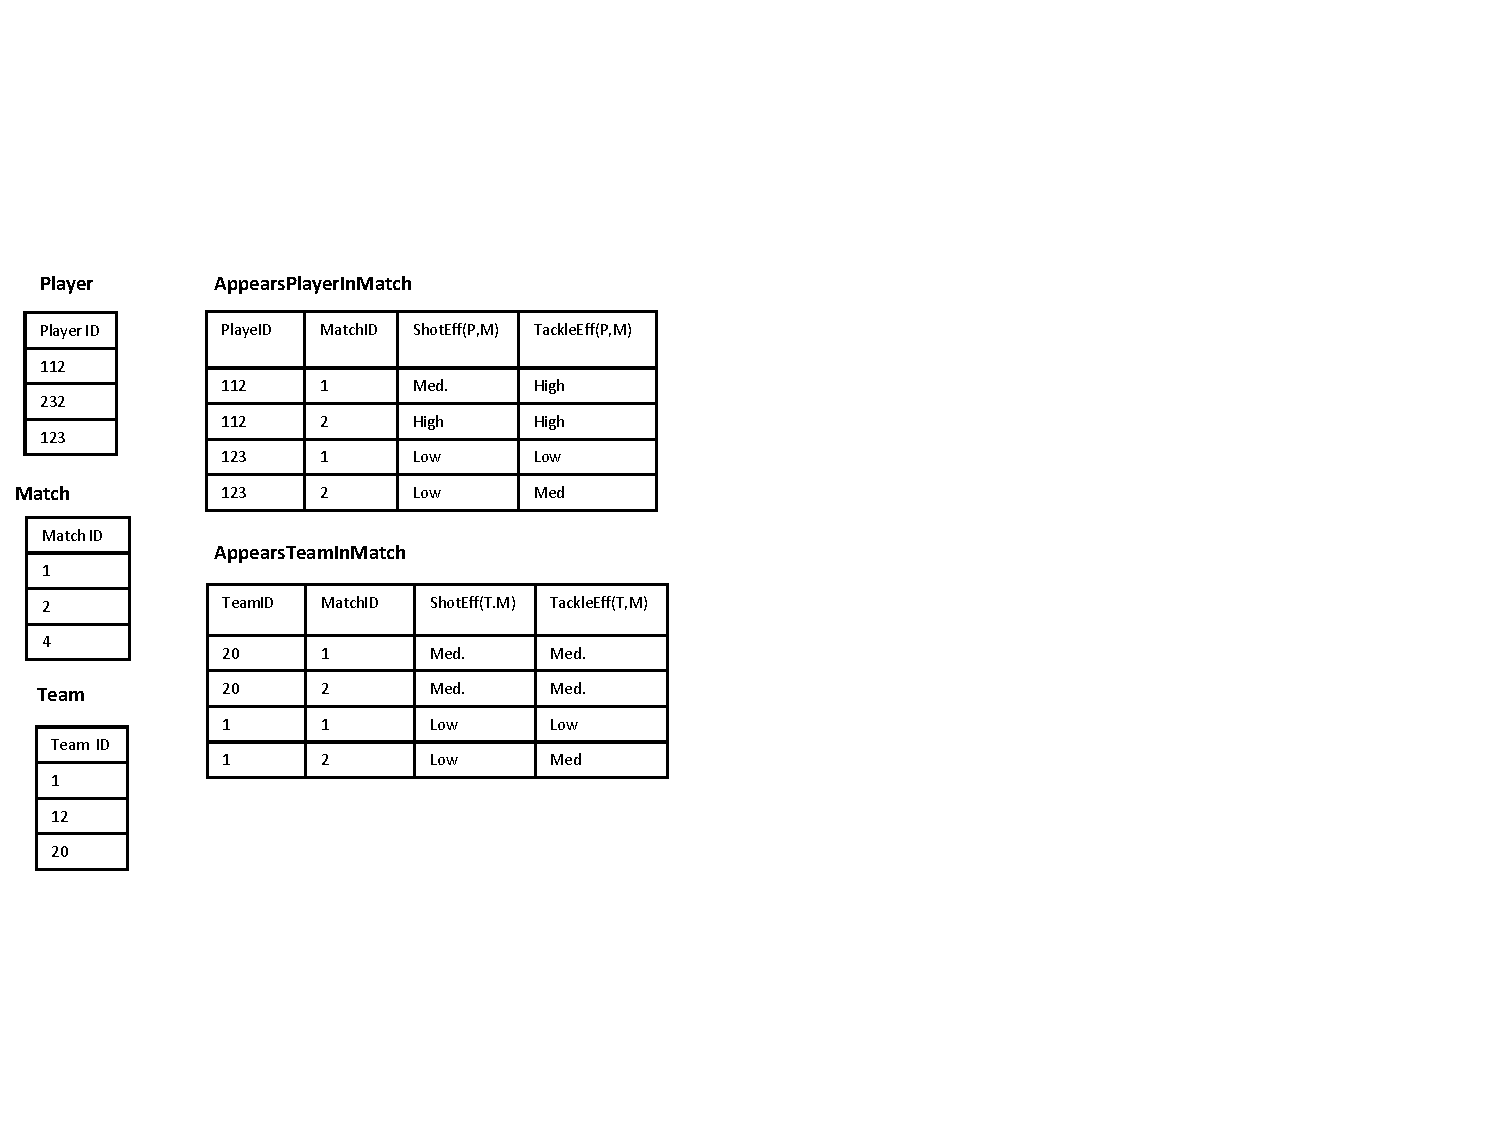
\includegraphics[scale=.6]{databasefigure.pdf}}
%	\end{minipage}%
%	\begin{minipage}{.55\linewidth}
%		\centering
%		\subfloat[The Propositionalization Pipeline]{\label{main:b}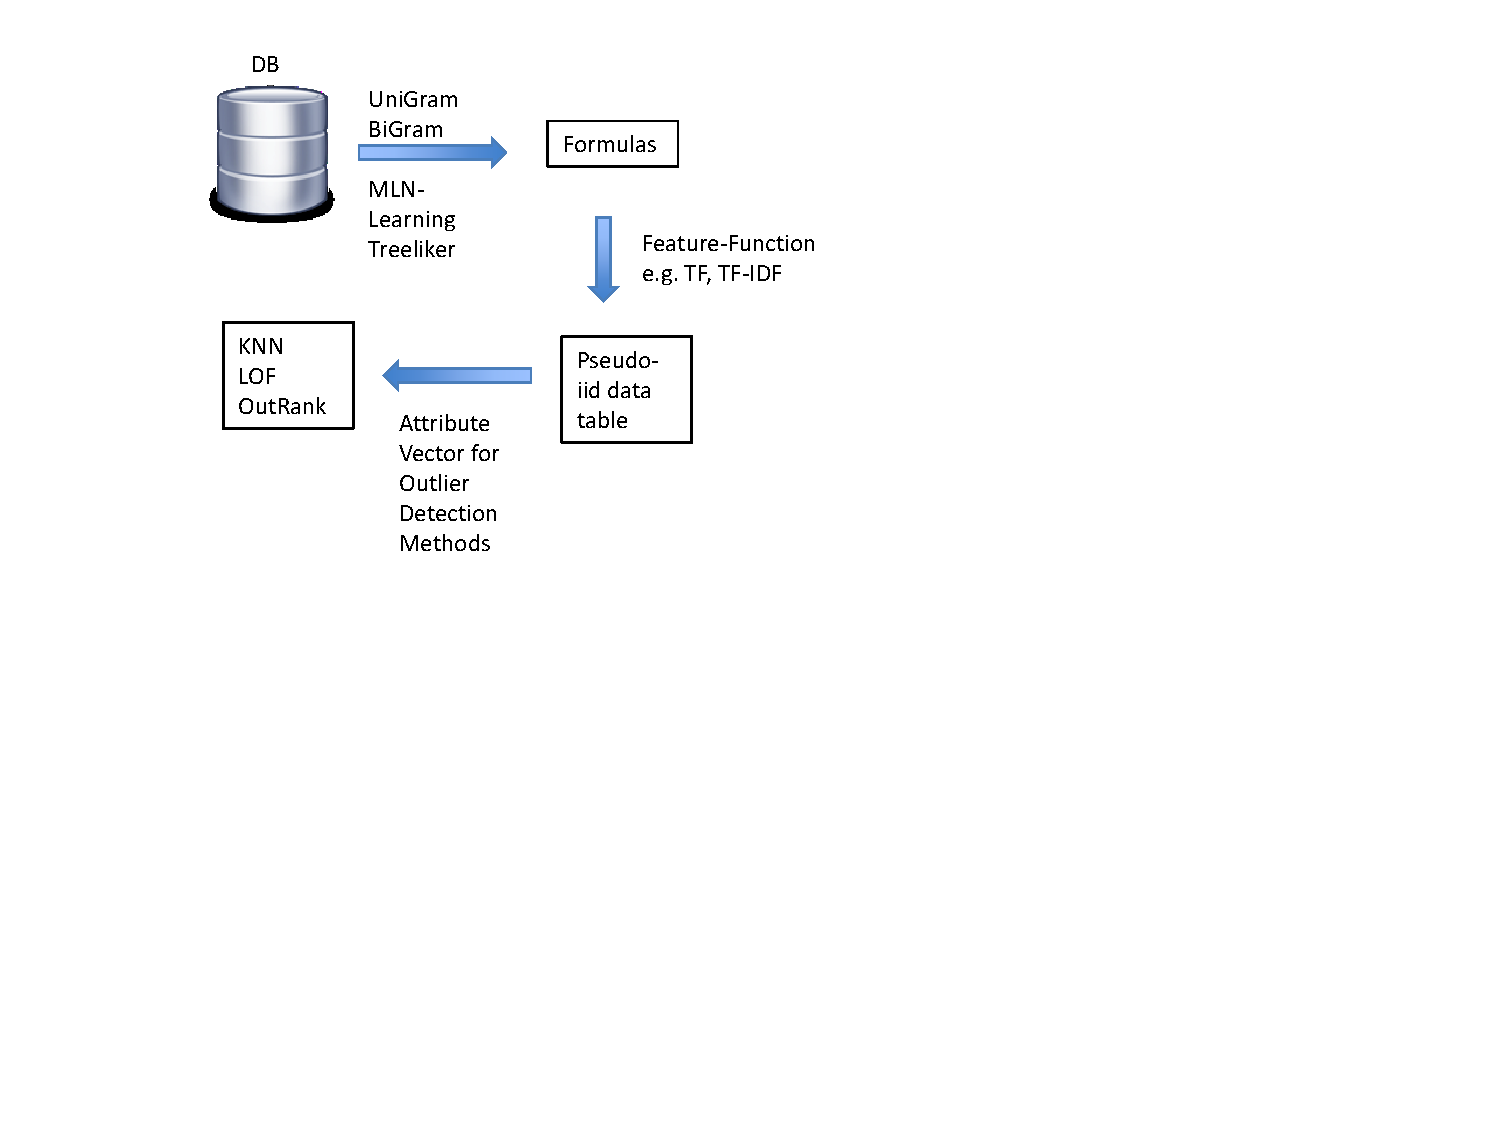
\includegraphics[scale=.45]{pipeline.pdf}}
%	\end{minipage}\par\medskip
%	\caption{System Flow}
%	\label{fig:propositionalize}
%\end{figure}

% We propose new methods for extending statistical  outlier detection to the case of object-relational data using a novel likelihood-ratio comparison for probabilistic models. 
%\paragraph{Markov Logic Network}~\cite{Domingos07} are one of the most well known methods of statistical relational learning. Essentially an MLN consists of a set of weighted first-order formulas that definesa Markov network comprising ground instances of logical predicates. The formulas are the structure of the network and represent associations between ground facts. The weights are the parameters of quantitative components and assign a likelihood to a given relational database by using the log-linear formalism of Markov networks. 
%
% 		\begin{table} 
% 			\caption{Example of a small MLN}
% 			\centering
% 			\resizebox{0.9\textwidth}{!}{
% 				\begin{tabular}{|c|c|l|}
% 					\hline
% 				First-order logic formula&Weight&Translation\\\hline
% 				$\forall(shotEfficiency(p)\rightarrow dribbleEfficiency(p))$&$w_{1}$&
% 					\begin{tabular}{p{3cm}} if shot efficiency of the player is high\\, dribble efficiency is high \end{tabular}\\\hline
% 					
% 					%Synthetic&40&280\\ \hline
% 				\end{tabular}}
% 			\end{table}
 \subsection{Approach}
 Many outlier detection methods have been developed for data that are represented in a propositional format (i.e., as a flat feature vector) or unstructured data.
 
 	\begin{figure*}[!h]
 		\centering
 		\resizebox{1\textwidth}{!}{
 			\includegraphics%[width=0.3\textwidth] 
 			{figures/MLN-Oct13.pdf}
 		}
 		\caption{Categorization of outlier detection methods. The bold font indicates where our methods stand in this categorization.
 			\label{fig:relatedWork}}
 	\end{figure*}
 In a propositional data table, a row represents a data point,
 a column represents an attribute of a data point, and a table entry represents
 an attribute value for a data point.\\
 This dissertation extends unsupervised statistical outlier detection to the case of structured data, more specifically object-relational data. Object-relational data represents a complex heterogeneous network~\cite{Gao2010}, which comprises objects of different types, links among these objects, also of different types, and attributes of these links. Given the prevalence of object-relational data in organizations, outlier detection for such data is an important problem in practice.
 However, applying standard outlier detection methods designed for single data tables on object-relational data runs into impedance mismatch, since object-relational data are represented in multiple interrelated tables.  
 
 In order to detect outliers in object-relational data, we have developed two generative model-based approaches. The advantages of employing a model-based approach for outlier detection task are as follows: 1) We can apply many statistical relational learning methods for building the model. 2) We can leverage statistical concepts such as divergence metrics to measure outlierness of the data points. 3) We can employ outlier detection methods designed for the propositional data.\\
  Based on Figure~\ref{fig:relatedWork} categorization, our proposed outlier detection methods fall into the category of unsupervised, relational learning-based, attributed models which can be applied to both static and dynamic datasets.

 \begin{enumerate}
 	\item In chapter~\ref{chap:four} a model-based method has been proposed to generate conjunctive features for outlier detection task. This method leverages outlier detection tools that are designed for the single table via a pipeline data preprocessing approach by converting the object-relational data into a single attribute-value table, then applying the data analysis tools. Since the attribute value representation corresponds to propositional logic, the conversion is called propositionalization. Propositionalization has been used to detect outliers in the literature. For example, a technique called ODDBALL introduced by Akoglue {\em et al.} extracts graph-centric features to detect anomalies in graph structure~\cite{Akoglu2010}. However, to the best of our knowledge, our work is the first model-based propositionalization approach for outlier detection. In chapter~\ref{chap:four} we show that conjunctive features for outlier detection can be learned from data by using statistical-relational methods. Specifically, we apply
 	Markov Logic Network structure learning method to construct the features. 
 	%
 	%Alternative propositionalization methods that we evaluate in this paper are based on enumerating all conjunctive formulas with at most two literals (unigrams and bigrams). 
 	Compared to baseline propositionalization methods, Markov Logic propositionalization produces the most compact data tables, whose attributes capture the most complex relational correlations. 
 	%(More complex correlations are represented by longer logical formulas). 
 	We apply three representative outlier detection methods ($\lof$, $\knn$, $\outrank$) to the data tables constructed by %Markov Logic 
 	propositionalization.\\
 	This research was published in the proceedings of the Florida Artificial Intelligence Association (FLAIRS2016) conference~\cite{Riahi2016}. 
 	\item Chapter~\ref{chap:five} introduces a model-based method to define outlierness metric. We first apply state-of-the-art probabilistic modelling techniques for object-relational data that construct a graphical model (Bayesian network), which compactly represents probabilistic associations in the data. We propose a new  metric, based on the learned object-relational model, that quantifies the extent to which the individual association pattern of a potential outlier deviates from that of the whole population. The metric is based on the {\em likelihood ratio} of two parameter vectors: One that represents the population associations, and another that represents the individual associations. 
 	Our method is validated on synthetic datasets and on real-world datasets about soccer matches and movies. Compared to the baseline methods, our novel likelihood-based model achieved the best detection accuracy on all datasets except one.
 	
 	Model-based methods have been previously used for outlier detection tasks. Loglikelihood has been used to identify outliers~\cite{Cansado2008}. Rule mining and sub-group mining are another examples of model-based outlier detection~\cite{Agrawal1994, Koh2005}. However, none of these methods are based on a joint distribution distance metric.
 	
 		This work was published in the proceedings of IEEE Symposium series on Computational Intelligence (SSCI 2015) conference and won the best student paper award~\cite{Riahi2015}.
 	
 	In chapter~\ref{chap:six} we compare the log-likelihood distance to metrics of success for a given domain. Success rankings are one of the most interesting features to users. Our reasoning is that high success is an independent metric that indicates an unusual individual. So a correlation between log-likelihood distance and success is an independent validation of the log-likelihood distance, and also shows that this metric points to meaningful and interesting outliers. A version of this work was submitted to the Journal of Data mining and Knowledge discovery.
 \end{enumerate}
   	Figure~\ref{fig:chap1-novelty} provides a tree picture of where our methods are situated with respect to other outlier detection methods and other data models.
   	
   		\begin{figure}
   			\centering
   			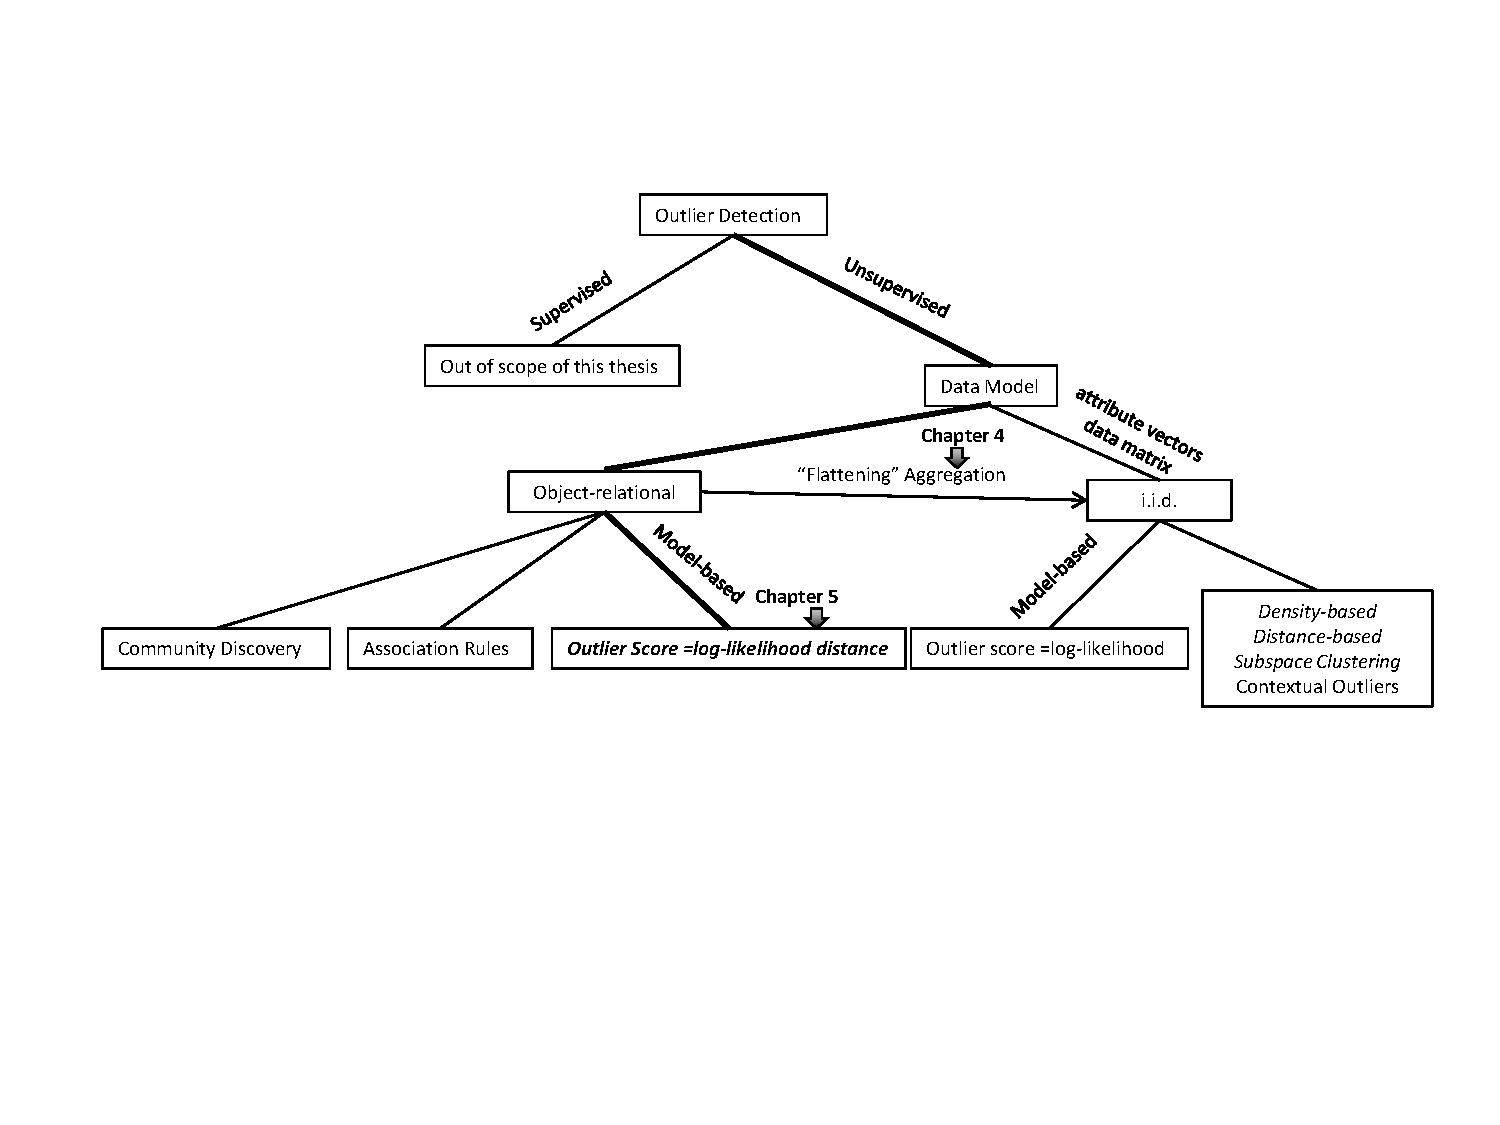
\includegraphics[width=1\textwidth] {figures/all-figures-chapter4-5.pdf}
   			\caption{A tree structure for research on outlier detection for structured data. A path specifies an outlier detection problem, the leaves list major approaches to the problem.
   				\label{fig:chap1-novelty}}
   		\end{figure} 
% In order to tackle the problem of outlier detection for the case of object-relational data, one possible approach is to leverage outlier detection tools that are designed for the single table via a pipeline data preprocessing approach: first, convert the multi-relational data into a single attribute-value table, then apply  the data analysis tools. Since the attribute value representation corresponds to propositional logic, the conversion is called propositionalization.
% %This can be done by to using Markov Logic Network (MLN) structure learning to learn set of formulas from the object-relatinal data and then use these formulas to construct the attributes of the single data table .
% Another possible approach is to apply probabilistic modeling techniques for object-relational data to construct a graphical model that represents normal behavior. An individual is deemed an outlier if the model assigns sufficiently low likelihood to generating its features.
 
%In this dissertation, we address three closely related research problems.
%\begin{enumerate}
%	 \item In Chapter~\ref{chap:four}, We develop a novel propositionalization  approach to unsupervised outlier detection for multi-relational data. Propositionalization summarizes the information from multi-relational data, that are typically stored in multiple tables, in a single data table. The columns in the data table represent conjunctive relational features that are learned from the data. An advantage of propositionalization is that it facilitates applying the many previous outlier detection methods that were designed for single-table data. 
%	 %		Previous work employed propositionalization for classification; in this paper we develop propositionalization for outlier detection. 
%	 We show that conjunctive features for outlier detection can be learned from data using statistical-relational methods. Specifically, we apply
%	 Markov Logic Network structure learning. 
%	 %
%	 %Alternative propositionalization methods that we evaluate in this paper are based on enumerating all conjunctive formulas with at most two literals (unigrams and bigrams). 
%	 Compared to baseline propositionalization methods, Markov Logic propositionalization produces the most compact data tables, whose attributes capture the most complex multi-relational correlations. 
%	 %(More complex correlations are represented by longer logical formulas). 
%	 We apply three representative outlier detection methods ($\lof$, $\knn$, $\outrank$) to the data tables constructed by %Markov Logic 
%	 propositionalization.\\
%	  A preliminary version of this research was published in the proceedings of the Florida Artificial Intelligence Association(FLAIRS2016) conference~\cite{Riahi2016}. 
%	 we use Markov Logic Network (MLN) structure learning to construct a single /data table from multi-relational data. This is a novel application of MLN learning. The format of the resulting data table is an individual-centric representation~\cite{Lippi2011,Lavrac13}:  we assume that there is a target class of individuals to be ranked as potential outliers (e.g. soccer players or movies). A row in the data table represents attributes of an individual. Attributes are defined by logical first-order formulas~\cite{Lippi2011}. The more complex the formula, the more relational information are represented by the formula. 
%	 %A function maps an individual and a first-order formula to a real value that is the value of the attribute for the individual. For example, we use the number of instantiations or groundings of a formula as such a function. 
%	 %
%	 A Markov Logic Network structure is a set of formulas.  Our Markov Logic propositionalization method applies a previous MLN structure learning method to produce a set of formulas; these formulas define attributes for propositionalization. Our approach can be summarized by the equation
%	 
%	 \begin{quote}
%	 	Markov Logic Network Structure = Set of Formulas = Set of Attributes.
%	 \end{quote}
%	 
%	 A baseline comparison method is to enumerate all conjunctive formulas up to a fixed length $n$ as attributes for propositionalization.  This is an instance of the recent Wordification approach to propositionalization \cite{Lavrac13}. A preliminary version of this research was published in the proceedings of the Florida Artificial Intelligence Association(FLAIRS2016) conference~\cite{Riahi2016}. 
	 %	 \item Chapter 5 focuses on the applications of the outlier metric introduced in Chapter 3. One of the important application is to use it in order to rank the individuals. In the datasets used in this dissertation, results show strong correlations between the outlier metric and the success metrics that naturally exists in the data (e.g. salary of the players or standing of the team).
%	\item In chapter 4, we present a new statistical approach to unsupervised outlier detection. 
%	 An individual object is deemed an outlier if  the model assigns sufficiently low likelihood to generating it. 
%	 A class-model Bayesian network (BN) structure is learned with data for the entire population. The nodes in the BN represent attributes for links, of multiple types, and attributes of objects, also of multiple types. To learn the BN model, we apply techniques from statistical-relational learning, a  recent field that combines AI and machine learning \cite{SRL2007,Schulte2012,Domingos2009}. 
%	 The BN provides dimensionality reduction, in the sense that it leverages independencies to represent the data distribution with exponentially fewer parameters than a non-factorized parametrization. 
%	 Given a set of parameter values and an input database, it is possible to compute a {\em class model likelihood} that quantifies how well the BN fits the object data. The class model likelihood uses BN parameter values {\em estimated from the entire class data.} This  is a relational extension of the standard log-likelihood method for i.i.d. vectorial data, which uses the likelihood of a data point as its outlier score. %This can be adapted for object-relational data as follows.
%	 %The Bayes net structure represents the normal pattern of associations among links and attributes  by the well-known d-separation criterion: Two nodes are probabilistically independent if they are d-separated. 
%	 While the class model likelihood is a good baseline score, it can be improved by comparing it to {\em the object model likelihood}, which uses BN parameter values {\em estimated from the object data.}
%	 The {\em model log-likelihood ratio} (LR) is the log-ratio of the object model likelihood to the class model likelihood. This ratio quantifies how the probabilistic associations that hold in the general population deviate from the associations in the object data substructure.
%	 While the 
%	 likelihood ratio discriminates relational outliers better than the class model likelihood alone, it can be improved further by applying two transformations: (1) a mutual information decomposition, and (2) replacing log-likelihood differences by log-likelihood distances. We refer to the resulting novel score as the {\em log-likelihood distance}.	 %For example, for each soccer team, there is a team distribution over: the team's attributes, the team's results in matches, and the actions of the team's players in matches. 
%%	 Step 2: Given a set of object profiles, compute an outlier score that measures how the object's profile differs from the profiles of other objects in its class. We develop a probabilistic approach where:
%	 
%%	 \begin{quote}
%%	 	Object Outlier Score = Score between object distribution and class distribution
%%	 \end{quote}
%%	 
%%	 For each object, the object distribution is a joint distribution over the object's attributes and the attributes of related objects. The object distribution can be computed from counts in the object profile. The class distribution is the distribution of a randomly chosen object in the class. 
%	A preliminary version of this work was published in the proceedings of IEEE Symposium series on Computational Intelligence (SSCI 2015) conference and won the best student paper award~\cite{Riahi2015}. Later on, a more detailed version of this paper was submitted to the Journal of Data mining and Knowledge discovery.
%	
%	 \item In chapter 5, We compare the log-likelihood distance to metrics of success for a given domain. Success rankings are one of the most interesting features to users. Our reasoning is that high success is an independent metric that indicates an unusual individual. So a correlation between log-likelihood distance and success is independent validation of the log-likelihood distance, and also shows that it points to meaningful and interesting outliers. A version of this work was submitted to the Journal of Data mining and Knowledge discovery.
%	 
%	 
%%	  we address an interesting problem of estimating individuals abilities. The idea is to compare each individual ability with the whole population. In the case of soccer player, we form the population to be group of defenders or midfielders or strikers. We used the novel likelihood ratio metric that is introduced in Chapter 4 to quantify the extent to which the individual associate pattern deviates from that of whole population. In order to compute the likelihood ratio metric, we learned two models, A graphical model that represents the population associations pattern and another graphical model that represents the individual association pattern. We use meaningful and independent metrics
%%	 that are available in the data such as salary of a player and box office of a movie as ground truth in order to validate our estimation. An empirical evaluation on soccer and movie data shows a strong correlation between the likelihood ratio and success metric.
%\end{enumerate}

\subsection{Contributions}
The main contributions of this dissertation are the followings:
\begin{enumerate} 
	\item The first approach to outlier detection for structured data that is based on a probabilistic model. 
	\item A new model-based outlier score based on a novel model likelihood comparison, the log-likelihood distance.  % \footnote{Commented paper organization}
	\item A novel task for relational learning: MLN-propositionalization for outlier detection. This facilitates leveraging standard single-table outlier analysis methods for object-relational data.  This task is also a novel application of Markov Logic Network structure learning.
	\item  A novel task for relational learning: propositionalization for outlier detection. This facilitates leveraging standard single-table outlier analysis methods for object-relational data. We use Markove Logic Network (MLN) structure learning for propositionalization task. This is a novel application of MLN structure learning.
	
%	\item A novel application of Markov Logic Network structure learning to perform this task. MLN structure learning learns a compact yet expressive set of features from multi-relational data.
%	\item Our proposed methods rank potential outliers, but do not set a threshold for a binary identification of outlier vs. non-outlier.
\end{enumerate}
\subsection{Limitations and Directions for Future Work}
The main limitations of the work presented in this dissertation are the following:
\begin{enumerate}
	\item \textbf{Limitation of Approach:} 
	\begin{enumerate}\item Our proposed methods rank potential outliers, but do not set a threshold for a binary identification of outlier vs. non-outlier.
		 \item Our current Bayesian Network Learning method can only be applied to discrete data. Prior to learning the model, we take an extra step in data preprocessing and convert the continuous data into discrete which naturally causes some information loss. \item Our generative model-based methods learn a generic Bayesian network structure for the entire population, ignoring the subgroups that inherently exist in the real datasets, as a result, the detected outliers are global outliers. However, there are  more complex outliers that locally deviate from their subgroups and can be detected only by subgroup comparison. One direction for future work is to first detect subgroups in the population and then perform the outlier detection task.
%		 \item In our 
		\end{enumerate}
		\item \textbf{Limitation of Data Analysis: }
	
		In this dissertation, to simplify the outlier detection task, we used only part of the full information available in our rich datasets. The model-based outlier detection can be extended in future work to take advantage of the full information. 
			\begin{enumerate}
				\item In the Premier League dataset, players are naturally related to one another and modelling the interaction between players can be another way to detect anomalous players.
				The graph-based features, such as detecting near-clique nodes and star nodes, proved to be efficient in discovering patterns for anomaly detection task as shown in ODDBALL~\cite{Akoglu2010}.
					\item In this dissertation we did not use the temporal information available in the data. In the learning process we do not give a higher weight (importance) to the more recent action (performance) of an individual. This point is especially important when applying the methods to dynamic data or the data that are collected from long periods of time. 
			\end{enumerate}
		
		%However, this is not a limitation of our proposed outlier detection system.


	%	\item \textbf{Limitation of application: }
	%	\item {local vs global}
	%		\item In this dissertation, we only focus on the action of each individual. In learning the graphical model, we do not take into account the inter-dependencies that inherently exist between individuals for the same class. For example, in the Premier League dataset, players are naturally related to one another and modeling the interaction between players can be another way to detect anomalous players.
%	The connectivity-based features proved to be efficient in discovering patterns for anomaly detection task as shown in ODDBALL.~\cite{Akoglu2010}. %features related to extent of interaction between players are examples of such features in our datasets.
	%one useful piece of information that can be utilized in the future work is to model different groups of individuals to identify which ones usually perform best together.
%	 the information of which players usually work the best together or the other way. 

%	\item Our current Baysian Network Learning model can only be applied to discrete data. Prior to learning the model, we take an extra step in data preprocessing and convert the continuous data into discrete which naturally causes some information loss. 
%	\item In this dissertation we assume the structure of the learned Bayesian network is fixed and we learned the parameters for that fixed structure. 
%	\item In our learning process, we do not give a higher weight (importance) to the more recent action (performance) of an individual. This point is especially important when applying the methods to dynamic data or the data that are collected from long periods of time. 
%	\item We do not leverage domain knowledge in our modelling. There are some attributes that play more important roles in evaluating individuals of a specific class. For example in Soccer domain, the shot efficiency or number of goals scored by a strikers is more important compare to other attributes such as the dribble efficiency.
\end{enumerate}
%-dynamic nist , we didnt weight the recent history more than old ones. -action between two players



